% User guide: http://mirrors.ctan.org/macros/latex/contrib/bookcover/bookcover.pdf

\PassOptionsToPackage{dvipsnames}{xcolor}
\documentclass[
    a5paper,
    spinewidth=10mm,
    markcolor=black,
    %trimmed % Show only trimmed part!
    ]{bookcover}

%\bookcovertrimmedpart{front} % Trimmed part is the front cover
%\bookcovertrimmedpart{back} % Trimmed part is the back cover
%\bookcovertrimmedpart{spine} % Trimmed part is the spine 

\usepackage{fix-cm}
\usepackage[latin]{babel}
\usepackage{lipsum,microtype,GS1,qrcode}

% Couleurs personnalisées et graphiques TikZ
\usepackage[dvipsnames]{xcolor}
\usepackage{graphicx}
\usepackage{tikz}
\usetikzlibrary{calc}
\begin{document}

\begin{bookcover}


    \bookcovercomponent{normal}{front}{
        \begin{tikzpicture}[overlay,remember picture]
            \node[inner sep=0pt, anchor=north east] at ($(current page.north east)-(1.2cm,1cm)$) {
                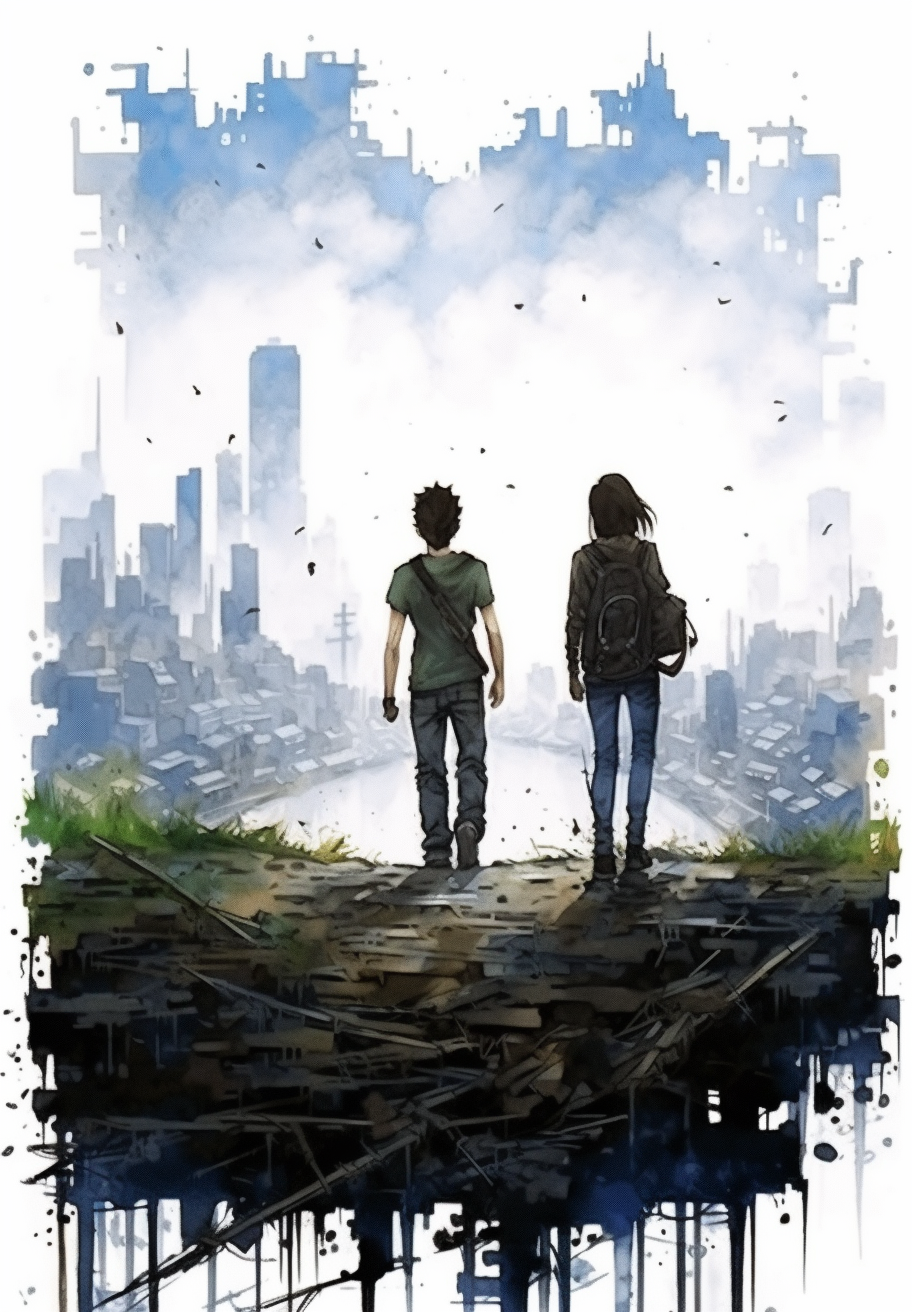
\includegraphics[width=170mm, keepaspectratio]{images/f6d72728-c5d7-4d9a-9c79-633bd48aeb30.png}
            };

            % Title
            \node[align=center] at ($(current page.north east)-(9.6cm,19.5cm)$)
            {
            {\fontsize{35}{72} \fontfamily{cmr}\selectfont \textcolor{white}{\textbf{En Quête d'Expérience}}}\\[0.5cm]
            {\fontsize{25}{72} \fontfamily{cmr}\selectfont \textcolor{white}{Le Chemin du.de la Jeune}}\\[0.25cm]
            {\fontsize{25}{72} \fontfamily{cmr}\selectfont \textcolor{white}{Développeur·euse}}
            };

            % Author
            \node[align=center] at ($(current page.north east)-(9.6cm,2.5cm)$)
            {
                {\fontsize{12}{19.2} \textcolor{black}{\selectfont {Kevin Delfour}}}\\[3pt]
            };
        \end{tikzpicture}
    }

    \bookcovercomponent{normal}{spine}[3mm,5mm,5mm,3mm]{
        \rotatebox[origin=c]{-90}{
            \fontfamily{cmr}
            \textbf{En Quête d'Expérience : Le Chemin du.de la Jeune Développeur·euse }
        }
        \vfill
        \rotatebox[origin=c]{-90}{
            \fontfamily{cmr} Kevin Delfour
        }
    }

    \bookcovercomponent{normal}{back}[22mm,10mm,22mm,30mm]{
        \begin{tikzpicture}[overlay,remember picture]
            \node[align=left, text width=120mm] at ($(current page.north)-(9.6cm,7.5cm)$)
            {
                {\fontsize{25}{72} \fontfamily{cmr}\selectfont \textcolor{black}{\textbf{En Quête d'Expérience}}}\\[0.5cm]

                \fontsize{13}{15} \fontfamily{cmr}\selectfont \textcolor{black}{
                    Ce livre est un guide destiné aux jeunes développeur·se·s souhaitant acquérir de l'expérience pour maximiser leurs chances de trouver un emploi.
                }\\[0.25cm]

                \fontsize{13}{15} \fontfamily{cmr}\selectfont \textcolor{black}{
                    Ce livre offre des conseils sur les différentes stratégies à adopter pour démontrer une certaine expérience et bien plus encore.
                }\\[0.25cm]

                \fontsize{13}{15} \fontfamily{cmr}\selectfont \textcolor{black}{
                    Il a pour objectif d'aider les développeur·se·s à mettre en place des actions concrètes qui leur permettront, par la suite, de justifier leur niveau d'expérience et leur passion lors de leur première recherche d'emploi.
                }\\[0.25cm]
            };

            \node[align=left, text width=120mm] at ($(current page.center)-(9.6cm,2.5cm)$)
            {
                {\fontsize{20}{72} \fontfamily{cmr}\selectfont \textcolor{black}{
                            \textbf{À propos de l'auteur}
                        }}\\[0.5cm]

                \fontsize{13}{15} \fontfamily{cmr}\selectfont \textcolor{black}{
                    Kevin Delfour est un développeur passionné et expérimenté qui a travaillé sur de nombreux projets dans divers domaines. Il partage ses connaissances et son expérience à travers ce livre pour aider les jeunes développeur·se·s à progresser dans leur carrière.
                }\\[0.25cm]
            };

        \end{tikzpicture}
    }

    \bookcovercomponent{normal}{back}[,1cm,,]{
        \vfill
        \centering
        \small{\textcolor{darkgray}{ISBN: 978-615-5297-19-9}}\\
        \small{\textcolor{darkgray}{Edition \textbf{{Le Vilain Petit Dev}}}}\\[0.5cm]


        \savebox0{
            \EANBarcode[module_height=15mm]{ISBN 978-615-5297-19-9}
        }
        \colorbox{white}{
            \usebox0
            \raisebox{\depth}{
                \qrcode[height=\ht0]{https://github.com/kdelfour/Ebook_The_path_of_the_young_developer_Your_quest_for_experience}
            }
        }
    }

    %\bookcovercomponent{ruler}{whole}{,,} % Check dimensions

\end{bookcover}

\end{document}